\documentclass[fleqn,a4paper,12pt]{article}
\usepackage[top=1in, bottom=1in, left=1in, right=1in]{geometry}


\usepackage{filecontents}

\begin{filecontents}{\jobname.bib}
\end{filecontents}


\title{深度學習應用——作業三報告}
\author{B03902072 江廷睿}
\date{}

\usepackage{listings}

\usepackage{amsmath}
\usepackage{amssymb}

\usepackage{graphicx}
\usepackage[margin=1cm]{caption}
\usepackage{subcaption}
\usepackage{float}

\usepackage{mathspec}
\setmainfont{Noto Serif CJK TC}
% \setmathsfont(Digits,Latin,Greek)[Numbers={Lining,Proportional}]{DejaVu Math TeX Gyre}
\newfontfamily\ZhFont{Noto Serif CJK TC}
\newfontfamily\SmallFont[Scale=0.8]{Droid Sans}
% \newfontfamily\SmallSmallFont[Scale=0.7]{Noto Serif CJK}
\usepackage{fancyhdr}
\usepackage{lastpage}
\pagestyle{fancy}
\fancyhf{}
\rhead{B03902072\ZhFont{江廷睿}}
\lhead{深度學習應用——作業三}
\cfoot{\thepage / \pageref{LastPage}}
\XeTeXlinebreaklocale "zh"

\renewcommand\tablename{表}
\renewcommand\figurename{圖}

\begin{document}
\maketitle
\thispagestyle{fancy}

\section{Describe your Policy Gradient \& DQN Model}

\subsection{Policy Gradient}

\subsubsection*{前處理}

\begin{itemize}
\item 忽略分數與底部的邊界,僅擷取遊戲畫面中間從從第 34 開始的 160 列像素。
\item 將紅色數值等於 144 或 109 的像素設成 0 ,以消除背景的顏色。
\item 使用亮度轉換公式將紅綠藍三色轉換成灰階
  \begin{equation*}
    \text{Luminance} = 0.2126 \times \text{R} + 0.7152 \times \text{G} + 0.0722 \times \text{B}    
  \end{equation*}
\item 使用 scipy.misc.imresize 這個函式把輸入縮小成 80 乘 80 的大小。
\item 減去上一個時間的處理後的影像。
\end{itemize}


\subsubsection*{網路架構}

使用如下的架構:

\begin{itemize}
\item 16 個捲積神經網路,kernel size (8, 8) , stride (4, 4)。
\item 線性整流函數。
\item 32 個捲積神經網路,kernel size (4, 4) , stride (2, 2)。
\item 線性整流函數。
\item 攤平成一維矩陣。
\item 神經元數量等於動作個數的完全連接層。
\item softmax 函數。
\end{itemize}

\subsubsection*{最佳化方式}

使用 RMSprop ,學習率等於 $10^{-4}$ 。

\subsection{DQN}

\subsubsection*{前處理}

直接使用助教提供的 wrapper 輸出的影像。

\subsubsection*{網路架構}

使用如下的架構:

\begin{itemize}
\item 32 個捲積神經網路,kernel size (8, 8) , stride (4, 4)。
\item 線性整流函數。
\item 64 個捲積神經網路,kernel size (4, 4) , stride (2, 2)。
\item 線性整流函數。
\item 64 個捲積神經網路,kernel size (3, 3) , stride (2, 2)。
\item 線性整流函數。
\item 攤平成一維矩陣。
\item 512 個神經元的完全連接層 。
\item 神經元數量等於動作個數的完全連接層。
\end{itemize}

\subsubsection*{最佳化方式}

使用 Adam ,學習率等於 $10^{-4}$ 。

\subsubsection*{演算法超參數}

\begin{itemize}
\item 獎勵的衰退 $\gamma$ :0.999 。
\item batch 大小:32 。
\item Replay buffer 大小:10000 。
\item 每次使用梯度上升更新網路的時間間隔: 4 步。
\item 同步參數到目標網路更新的間隔:每隔 5000 次更新,也就是 20000 步。
\item $\epsilon$-greedy 探索的參數 $\epsilon = \max(1 -  0.9 \cdot \frac{t}{400000}, 0.1 - 0.09 \cdot \frac{t}{4000000}, 0.01)$ ,其中 $t$ 為網路更新的次數。
\item 大約經過 700000 次更新後就可以有平均每次生命 60 分(原始分數)的成績。
\end{itemize}

\section{Plot the learning curve to show the performance of your Policy Gradient on Pong}

請參考圖 \ref{fig:learning-curve-pg} 。

\section{Plot the learning curve to show the performance of your DQN on Breakout}

請參考圖 \ref{fig:learning-curve-dqn} 中綠色的曲線。

\begin{figure}[h]
\centering
\begin{subfigure}{.45\textwidth}
  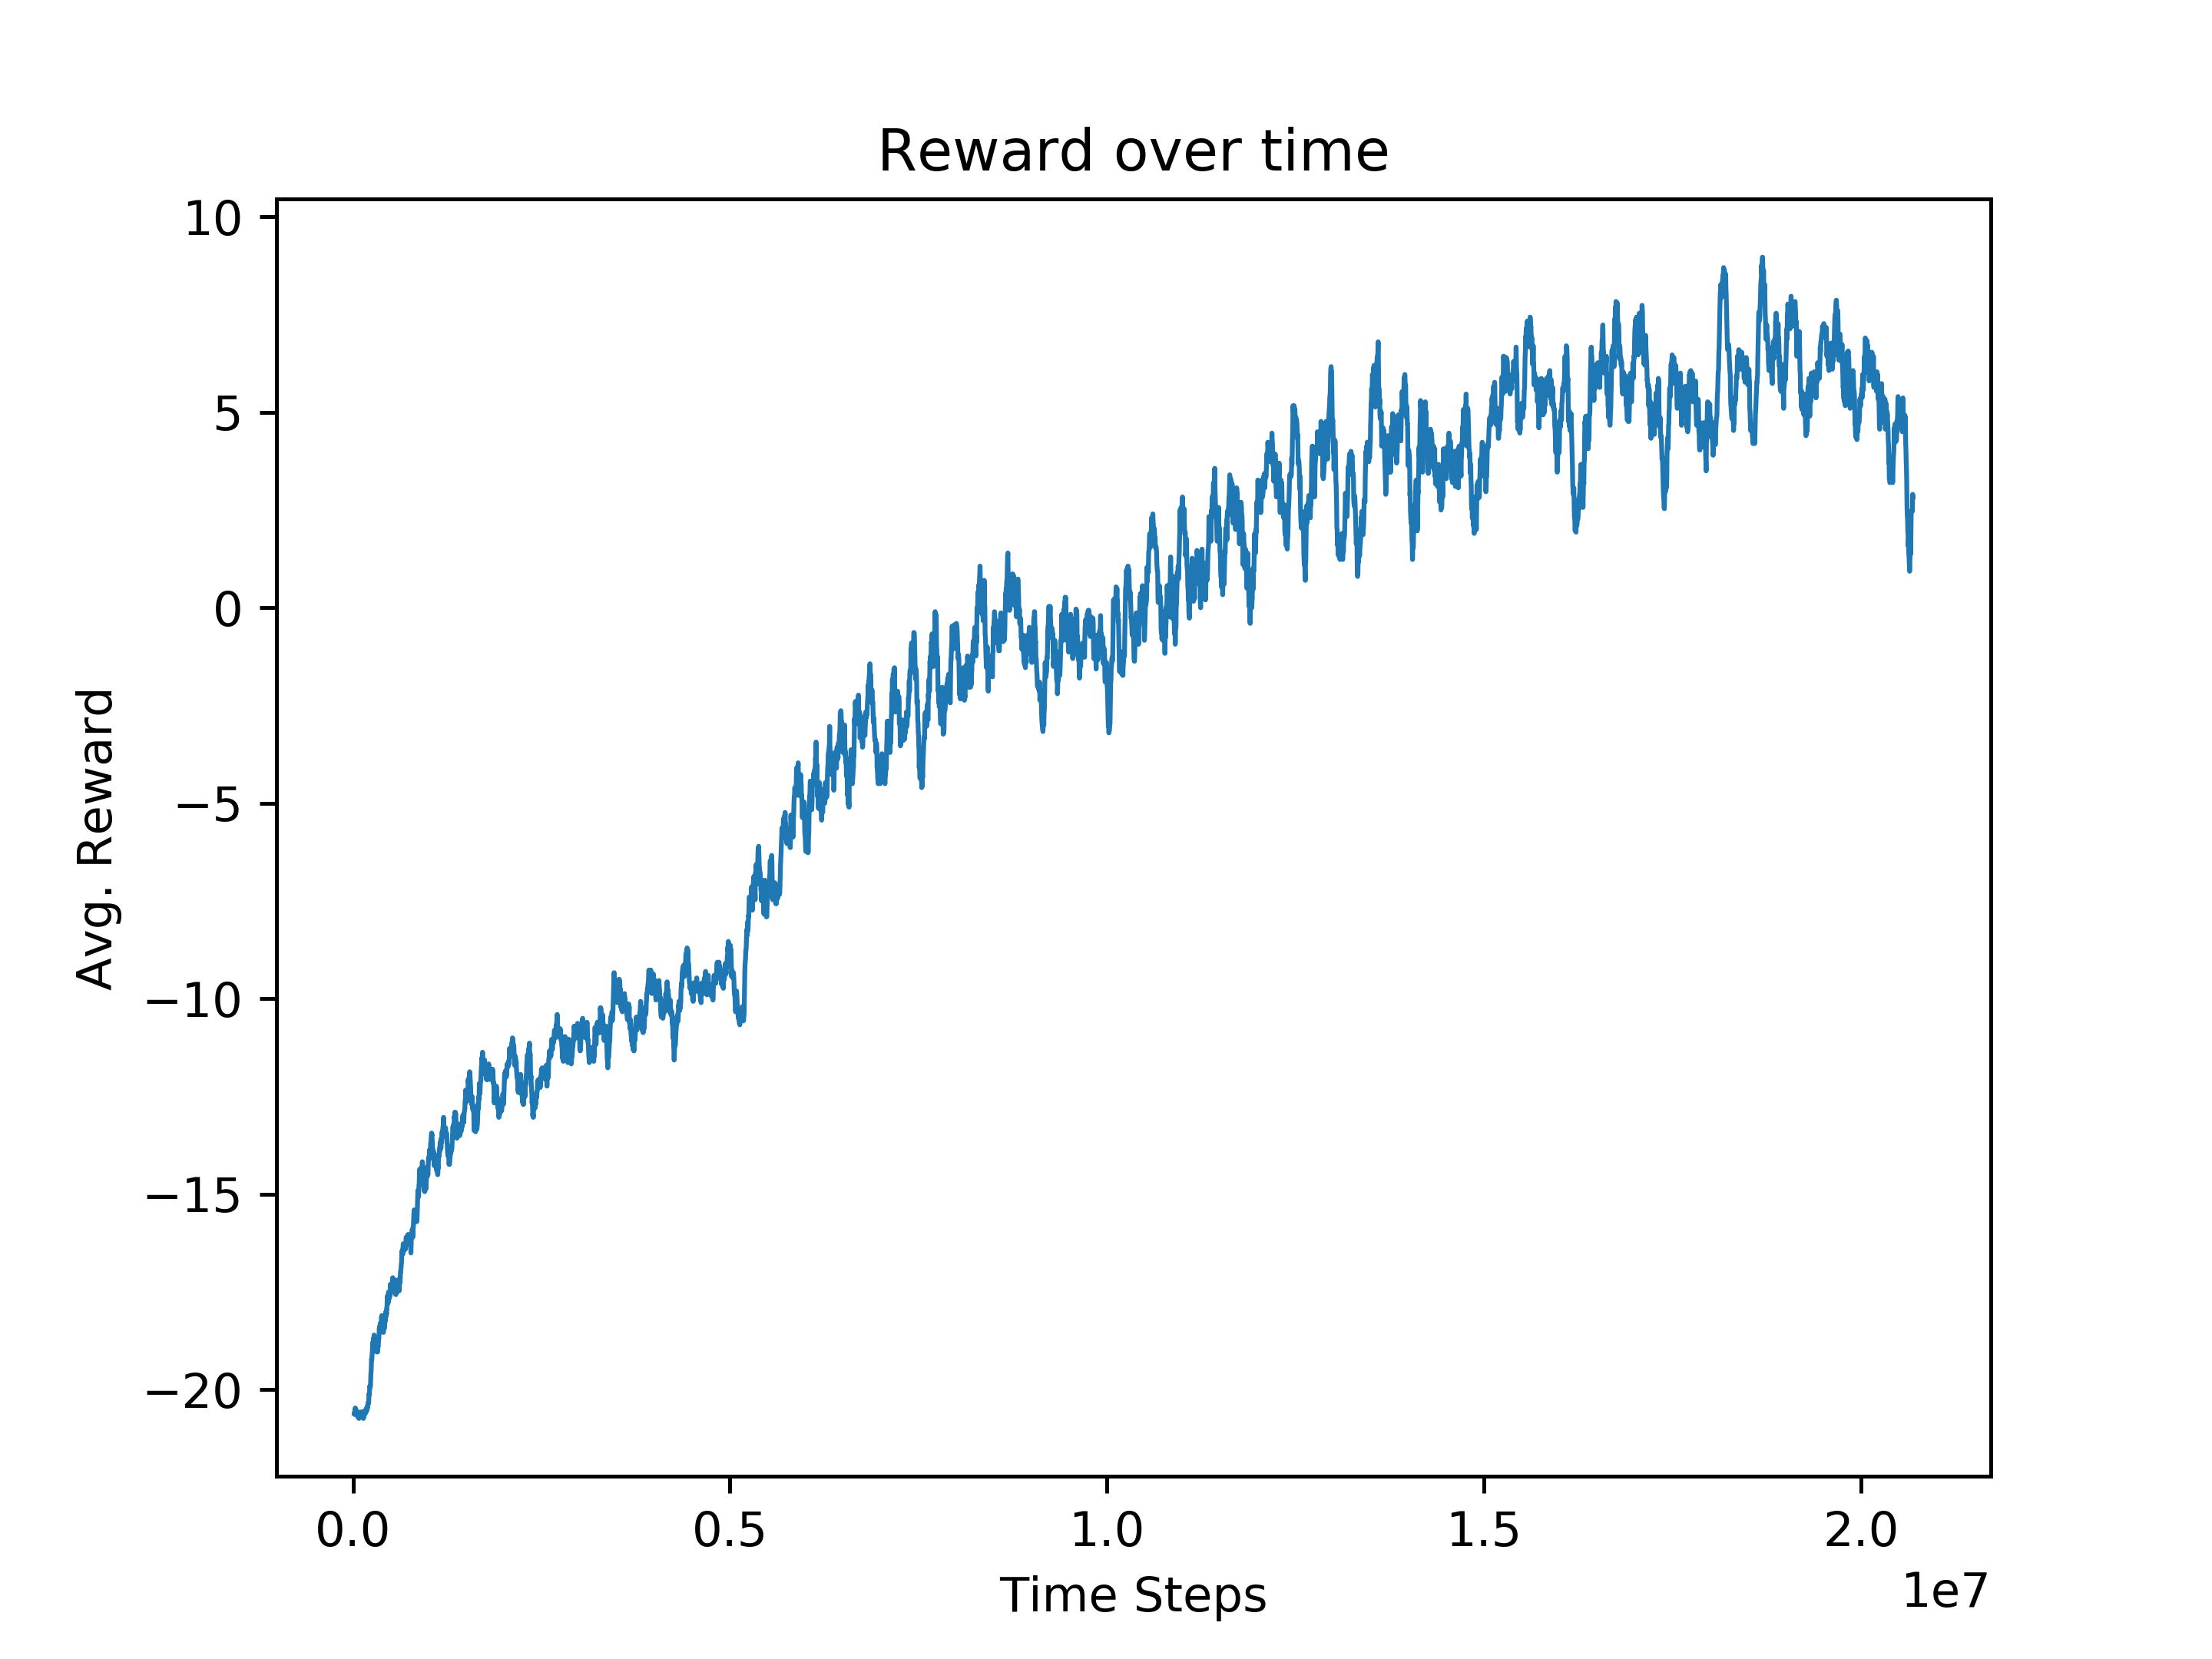
\includegraphics[width=\linewidth]{figures/pg.png}
  \caption{Atari 遊戲 Pong 每 30 場遊戲(21 分)平均分數(贏球數減輸球數)與訓練時間}
  \label{fig:learning-curve-pg}
\end{subfigure}
\begin{subfigure}{.45\textwidth}
  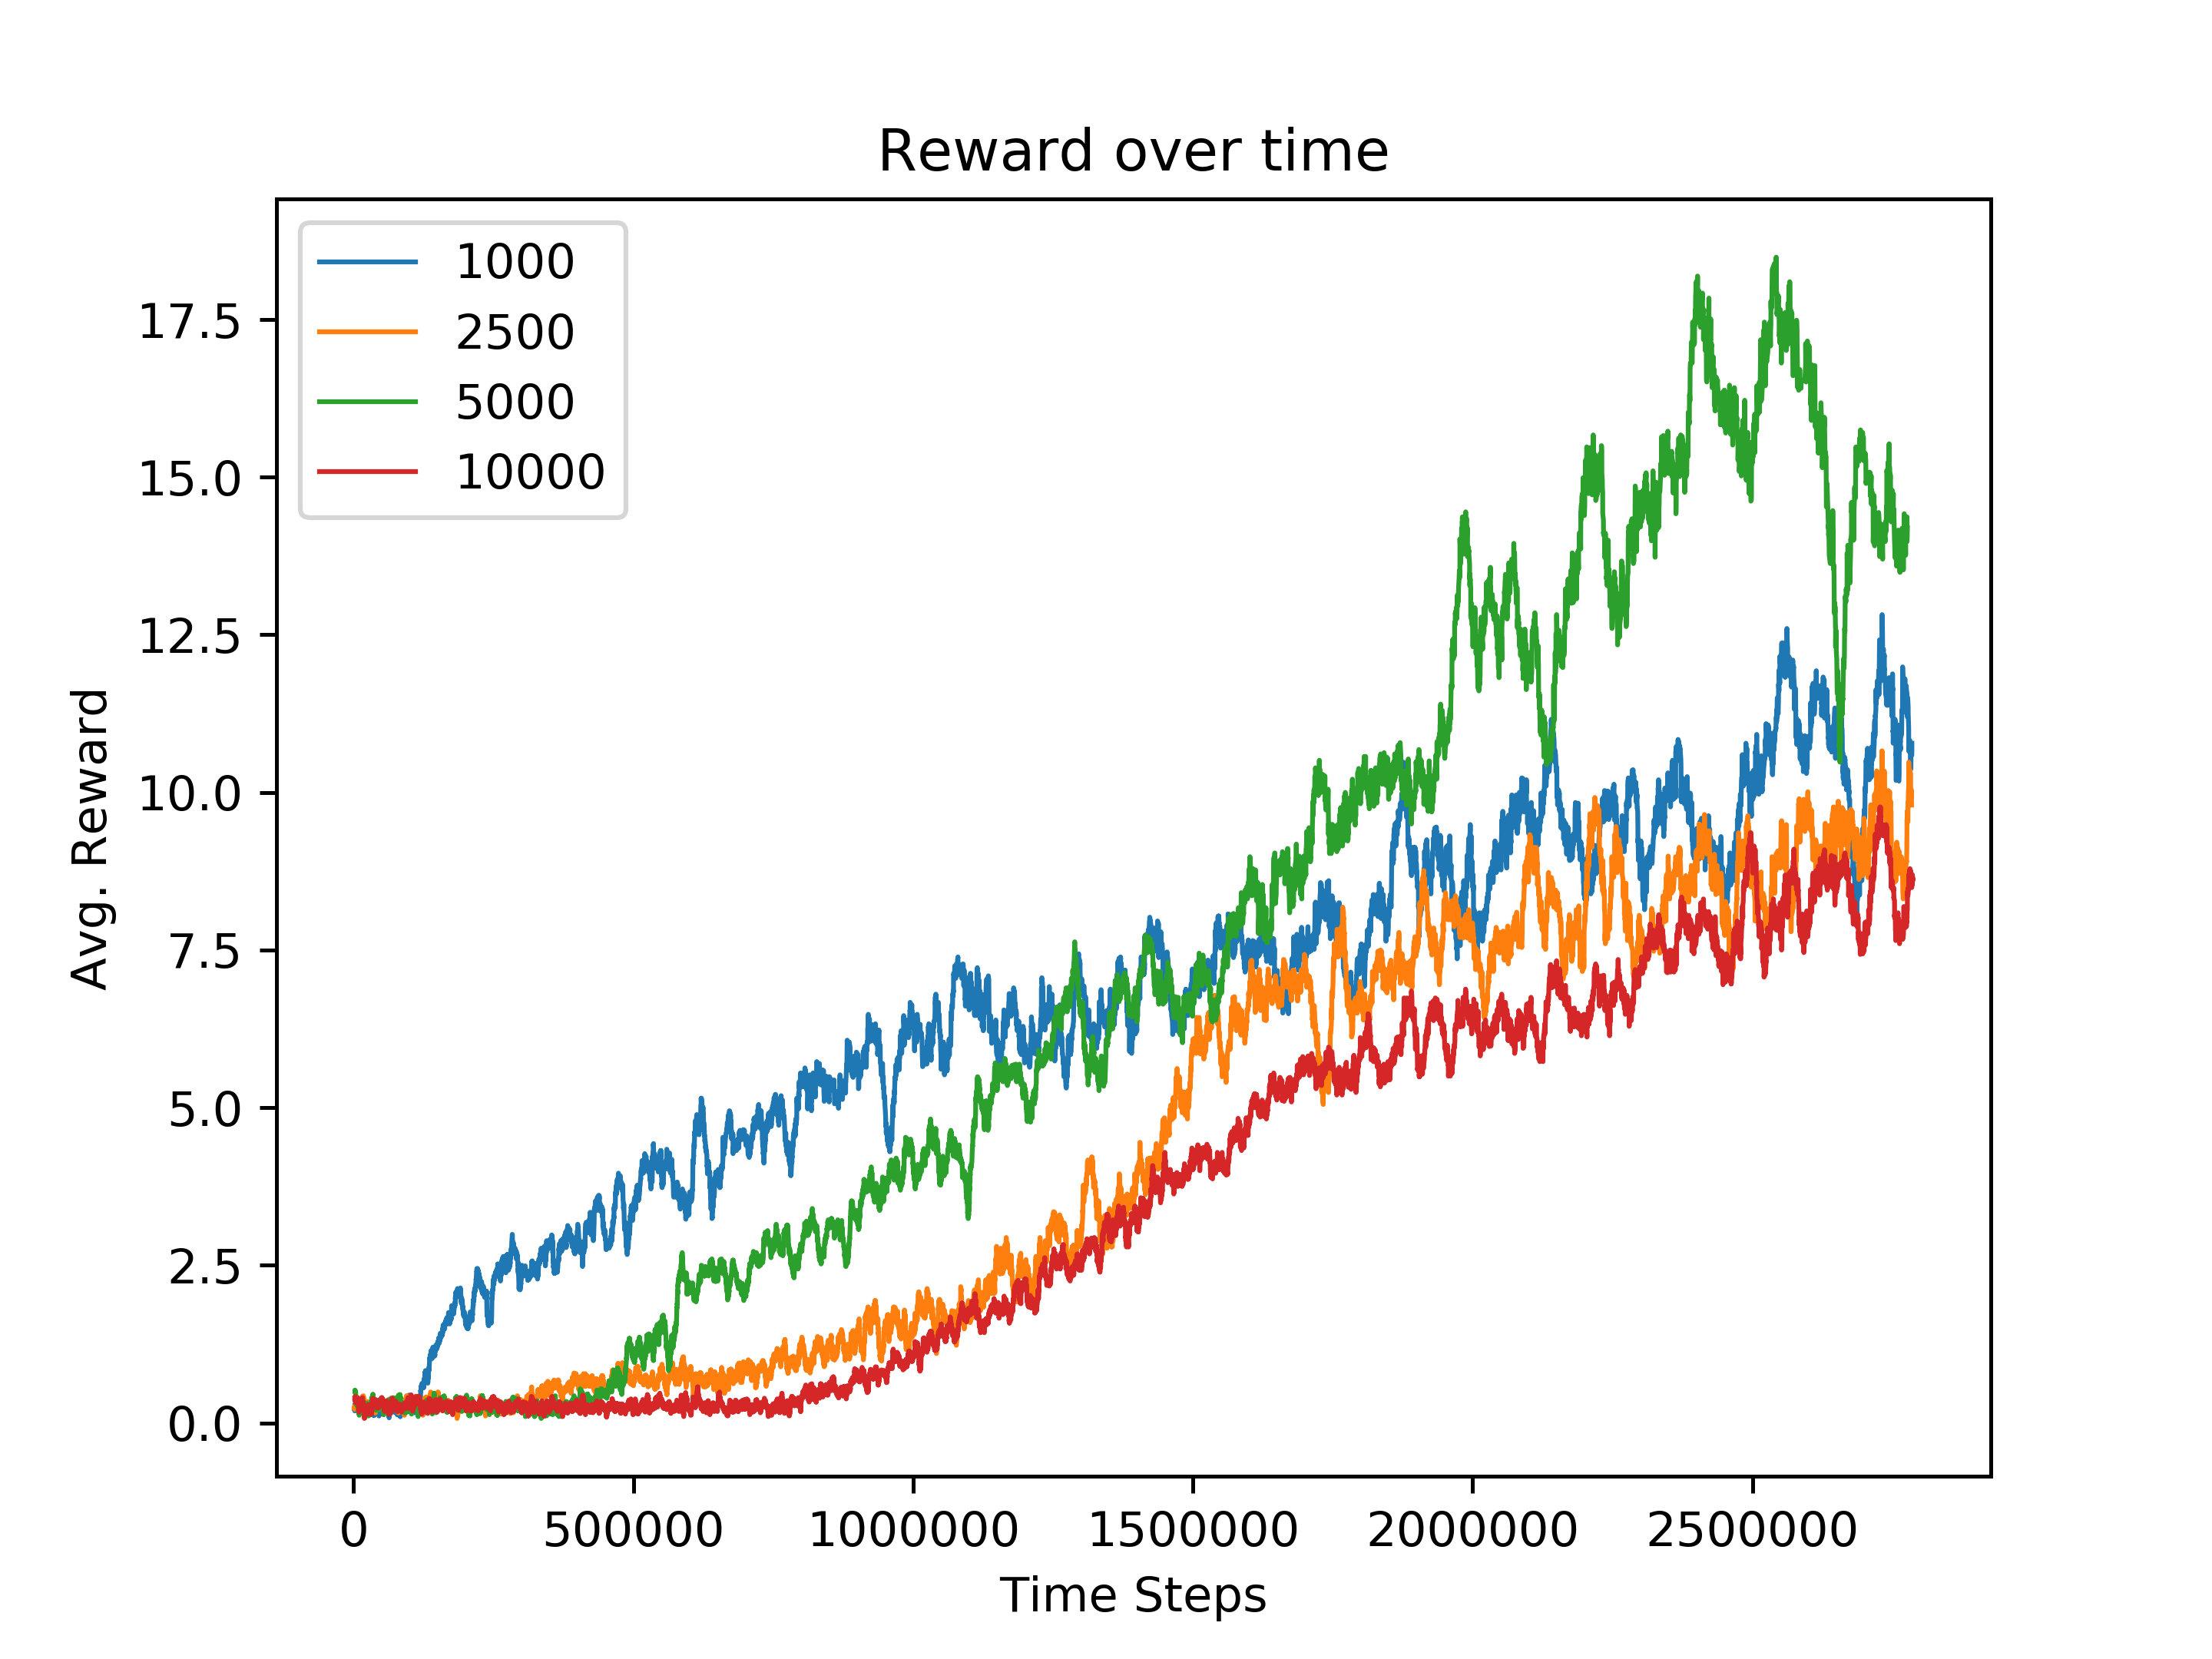
\includegraphics[width=\linewidth]{figures/dqn-update-freq.png}
  \caption{Atari 遊戲 Breakout 每 100 場遊戲(一條命)平均撞擊磚塊數量與訓練時間}
  \label{fig:learning-curve-dqn}
\end{subfigure}
\label{fig:learning-curve}
\caption{Policy Gradient 與 DQN 的學習曲線}
\end{figure}


\section{Experimenting with DQN hyperparameters}

這裡選擇實驗同步參數到目標的時間間隔。會選擇這個參數是因為理論上較長的間隔可以保證比較平穩的訓練效果,過小的間隔可能會導致網路沒有足夠的樣本學習到當前動作預期獎勵。然而因為 TD-loss 的性質,推測網路可以預測出的最大值也會受限於目標網路更新的次數,所以過長的間隔也會延遲網路預測較大數值的時間,進而延遲模型發展出長遠規劃的能力。實際實驗後,參考圖 \ref{fig:learning-curve-dqn} ,若是每隔 1000 次更新就同步一次,則一開始可以有比較快速的成長,但之後的成長速度就不及每隔 5000 次的綠色曲線。而若是每個 10000 次更新才同步一次,則是可以看到它上升的速度顯著的比其餘三者慢,但長遠來看說不定會更加穩定。

\section{Improvements to Policy Gradient}

\section{Improvements to DQN}

這邊試著使用 Double-DQN 和 Prioritized Replay Buffer 實驗在 Atari 的遊戲 Atlantis 上。\\

Double-DQN 主要是為了解決 DQN 容易高估數值。原先的 DQN 因為都是選擇最大的數值,所以即使模型的預測錯誤也有可能偏低,但往往都是偏高的被考慮到,從而累積出更大的錯誤。Double-DQN 提出了在計算目標數值時,不要使用預測數值的網路選擇最好的動作,並證明了如此一來 Double-DQN 將不會高估。實做上,也就是在計算目標數值時使用線上的參數:

\begin{equation*}
  Y_{target} = R_t + \gamma Q_{target}(s_{t+1}, \arg \max_a Q(s_{t+1}, a))
\end{equation*}


Prioritized replay 則是改變過去的經驗在用來訓練網路時被取樣到的機率分佈,使得過去有較高預測錯誤的樣本更容易被取樣到,達到加快訓練速度的效果。\\

參考圖 \ref{fig:learning-curve-dqn-atlantis} ,在實際實驗的學習曲線中,可以看到 DDQN 比 DQN 更快的到達更好的水準,而使用 prioritized replay 的 DQN 則是在前段時間大致上都有比其餘兩者更好的表現。至於為什麼使用 prioritized replay 的 DQN 為什麼在之後沒有比 DQN 更好,推測有可能是 prioritized replay 的超參數需要進一步的調整,或是 replay buffer 的大小需要更大,不過這部份就沒有繼續實驗。

\begin{figure}[h]
  \centering
  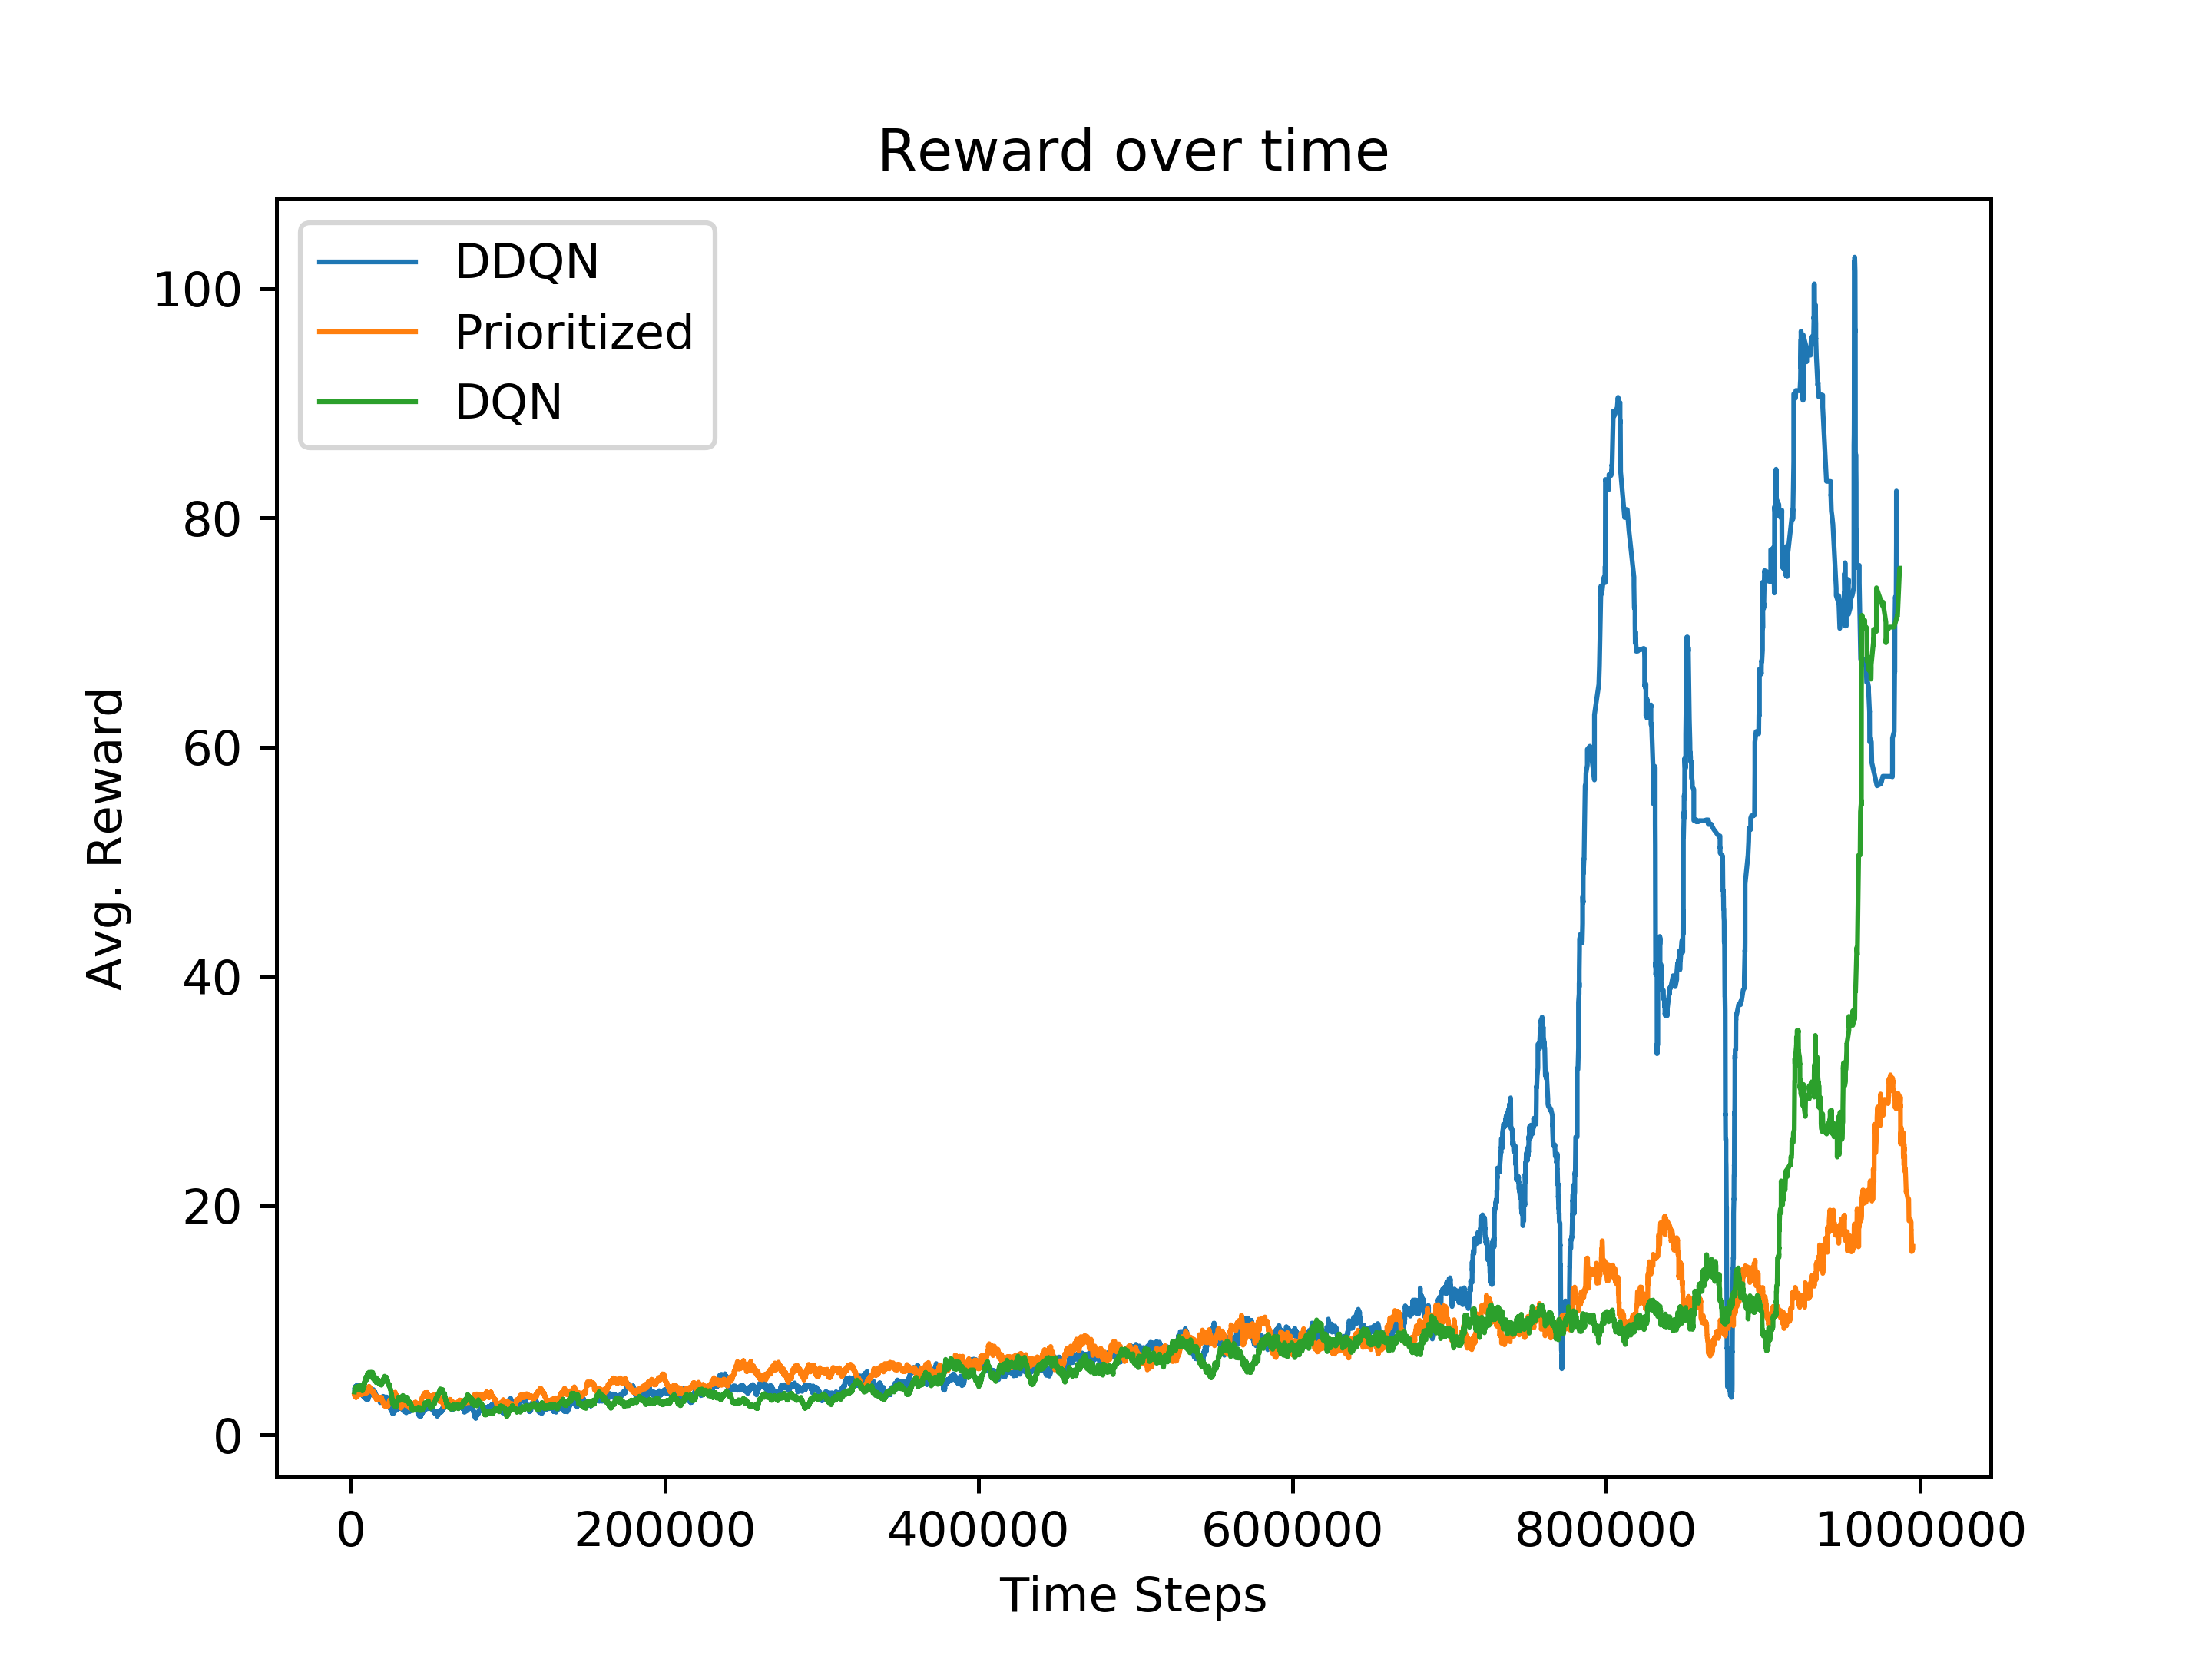
\includegraphics[width=0.9\textwidth]{figures/atlantis.png}
  \caption{DQN 在 Atlantis 上的學習曲線}
  \label{fig:learning-curve-dqn-atlantis}
\end{figure}

\bibliographystyle{ieeetr}
\bibliography{\jobname}

\section{Other RL method: Actor Critic}

一般的 Policy Gradient (REINFORCE Algorithm) 每次遊戲只能更新一次參數,對於經驗的使用效率非常不高。Actor Critic 結合了預測獎勵的 value function ,可以不用等到遊戲結束才能更新參數,所以理論上可以訓練的比較快。這邊試著實做了 Actor Critic 的演算法,每 32 步就更新一次 policy network 與 value network

\begin{align*}
  & \theta^{\pi} \leftarrow \theta^{\pi} + \eta \nabla \mathcal{R}(\theta^\pi) \\
  & \nabla \mathcal{R}(\theta^\pi) = \sum_t (\mathrm{Return}(s_t) - V^\pi(s_t)) \nabla \log p(a_t | s_t, \theta^\pi) \\
  & \mathrm{Return}(s_t) = r_t + V^\pi(s_{t+1}) \\
  & \theta^{V} \leftarrow \theta^{V} + \eta \nabla V(\theta^V) \\
  & \nabla V(\theta^V) = \nabla (V(s_t) - (r_t + \gamma V(s_{t+1})))^2 
\end{align*}

其學習曲線如圖 \ref{fig:learning-curve-actor-critic} 。在圖中可以看到,在訓練過程後期的某個時間開始,分數不升反降。這推測有可能是因為這個 Actor Critic 沒有加入 replay buffer ,或是出現了一些數值上不穩定的狀況產生。

\begin{figure}[h]
  \centering
  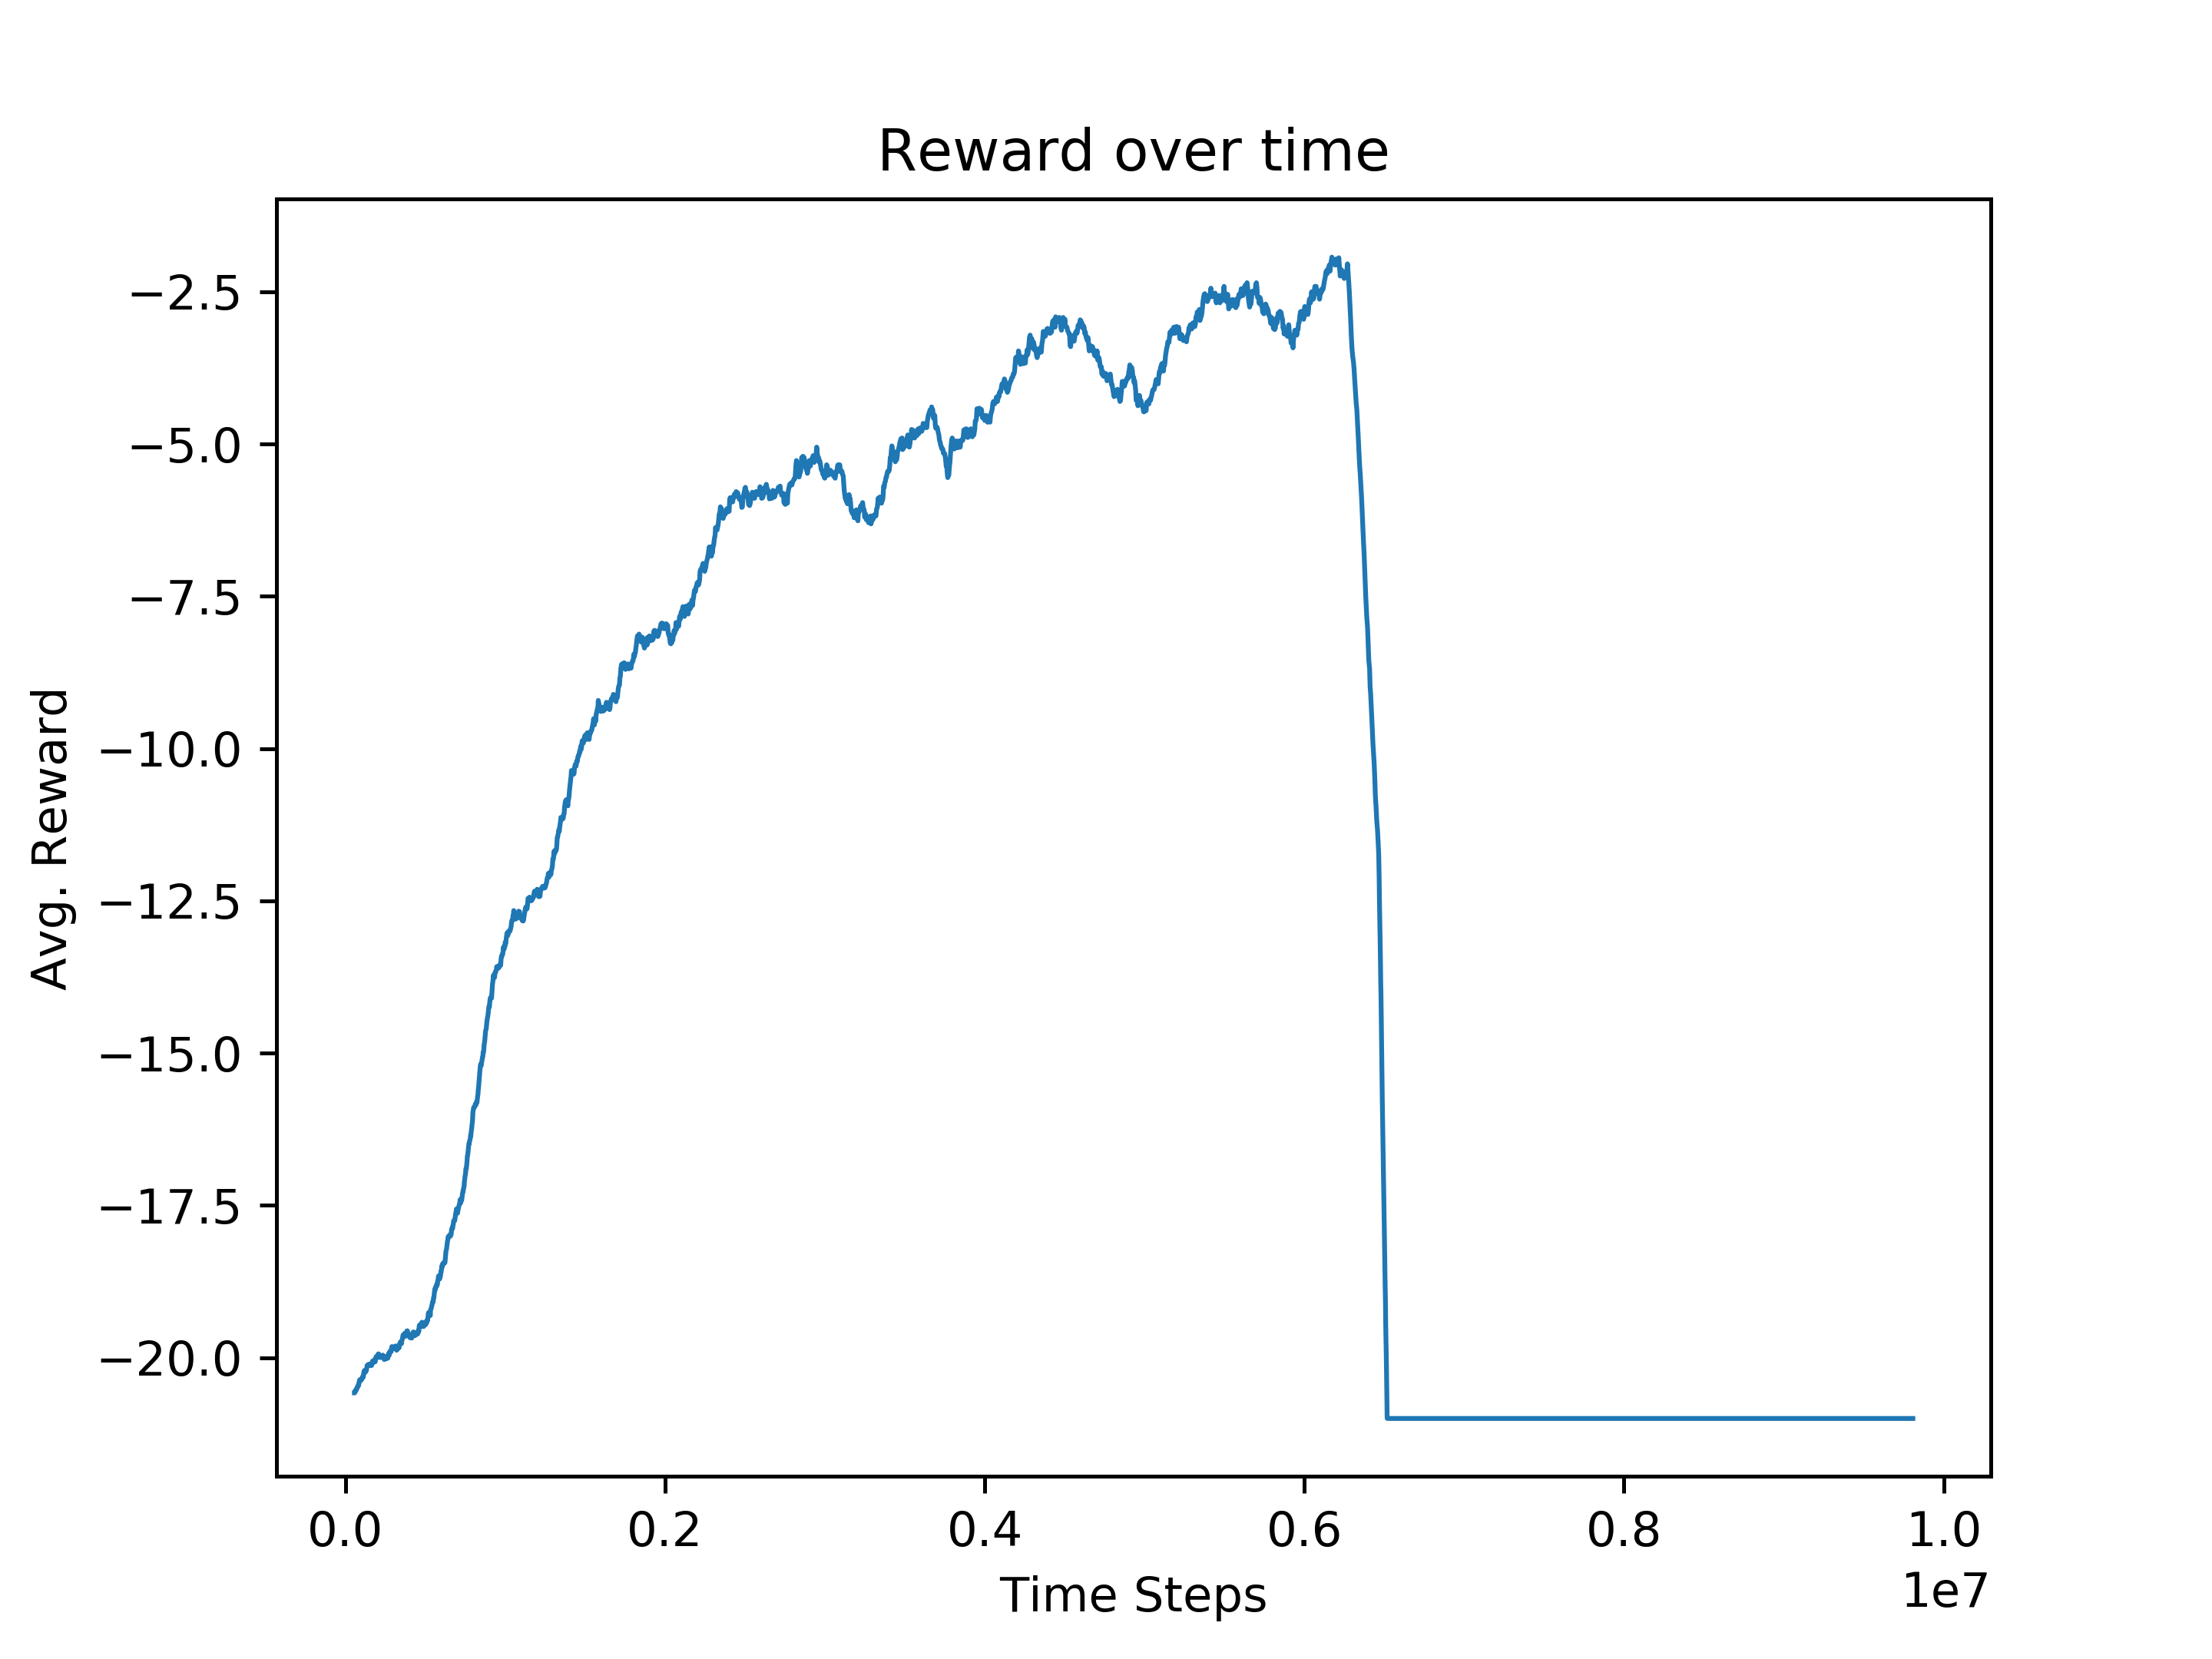
\includegraphics[width=0.9\textwidth]{figures/actor-critic.png}
  \caption{Actor-Critic 在 Pong 上的學習曲線}
  \label{fig:learning-curve-actor-critic}
\end{figure}


\end{document}
